% \begin{savequote}[8cm]
% \textlatin{Neque porro quisquam est qui dolorem ipsum quia dolor sit amet, consectetur, adipisci velit...}

% There is no one who loves pain itself, who seeks after it and wants to have it, simply because it is pain...
%   \qauthor{--- Cicero's \textit{de Finibus Bonorum et Malorum}}
% \end{savequote}

% Proposed old structure (pre-separation into RW and context):
% Global Scholarship Programs
    % A (Recent) History of Global Scholarship Programs
    % The Specific Programs we Work With
    % New and Pressing Selection Problems for these Programs
% Unsolved Problems in Talent Selection
    % Social considerations and the central selection problem
    % Modern Evaluation and the Problem of Generative AI
    % Fair Selection Across Locales
    % The Social and Organisational Value of Diversity
% Existing Quantitative Decision Support Approaches

% New structure is something like:
% Decision Support Tools
% Generative AI Detectors
% Explainable AI
% Quantitative Modelling for Diversity


\chapter{\label{ch:rw}Decisions in the Global Talent Selection Context} 
\minitoc

\section{A (Recent) History of Global Scholarship Programs}
\section{Programs we Work With}\label{ssec:programs}
\subsection{Foreword}
We work with two global scholarship and talent investment programs: the Ellison Scholars Program and the Rise Program. Both programs have asked that they not be identified in public facing research, and thus we request that reviewers not share details on Section \ref{ssec:programs} or knowledge contained within. Throughout the remainder of this Thesis, we refer to the Ellison Scholars Program and the Rise Program as Program A and Program B, respectively. However, to provide reviewers with the context and detail required to appropriately evaluate this work, we provide a brief overview of each program in this section.

\subsection{The Rise Program}\label{ssec:rise}
\subsubsection{Program Overview}
Initiated from a $\$1$-billion investment, Schmidt Futures and the Rhodes Trust's Rise program\footnote{https://www.risefortheworld.org/} finds and selects talented and disadvantaged 15-to-17-year-olds from around the world and helps them achieve their full career and service potential. Rise supports selected `winners' and `finalists' with a variety of benefits accessible at different points in their life. We work with Rise from the program's inception in 2021 until 2024. In each of these years, Rise has made a commitment to select up to 100 winners and up to 500 finalists from their pool of applicants. In the four applications cycles between 2021 and 2024, during which time Rise has selected 400 winners and nearly 2000 finalists from hundreds of thousands of started applications.

Rise uses a flexible benefits model, where winners (and, in some cases, finalists) gain access to a variety of potential resources, but utilise only resources they demonstrate need of. For example, applicants who recieve full scholarships to their university may not recieve an academic scholarship from Rise. Program benefits include academic scholarships, educational resources and programs, networking opportunities, and even funding for winner-led startups.\footnote{As academic scholarships comprise a large portion of program benefits, we speak about Rise as a ``scholarship and talent investment'' program throughout. This is our own language, and is intended to further anonymise the program. Similarly, we replace the program-specific term ``winners'' with ``scholars''.}

\subsubsection{The Selection Process}
The program uses a two-stage selection process designed to be accessible to candidates various global and socioeconomic backgrounds. In stage one, applicants submit various application materials asynchronously; Rise selects up to 500 finalists based on the quality of those materials and the program's cohort composition goals. In stage two, finalists engage in one of several ``finalist days'' consisting of various collaborative live activities and an interview; after all finalist days are completed, Rise uses information from both stages to select 100 winners.

\begin{figure}[htbp]
    \centering
    \begin{subfigure}{.45\textwidth}
        \centering
        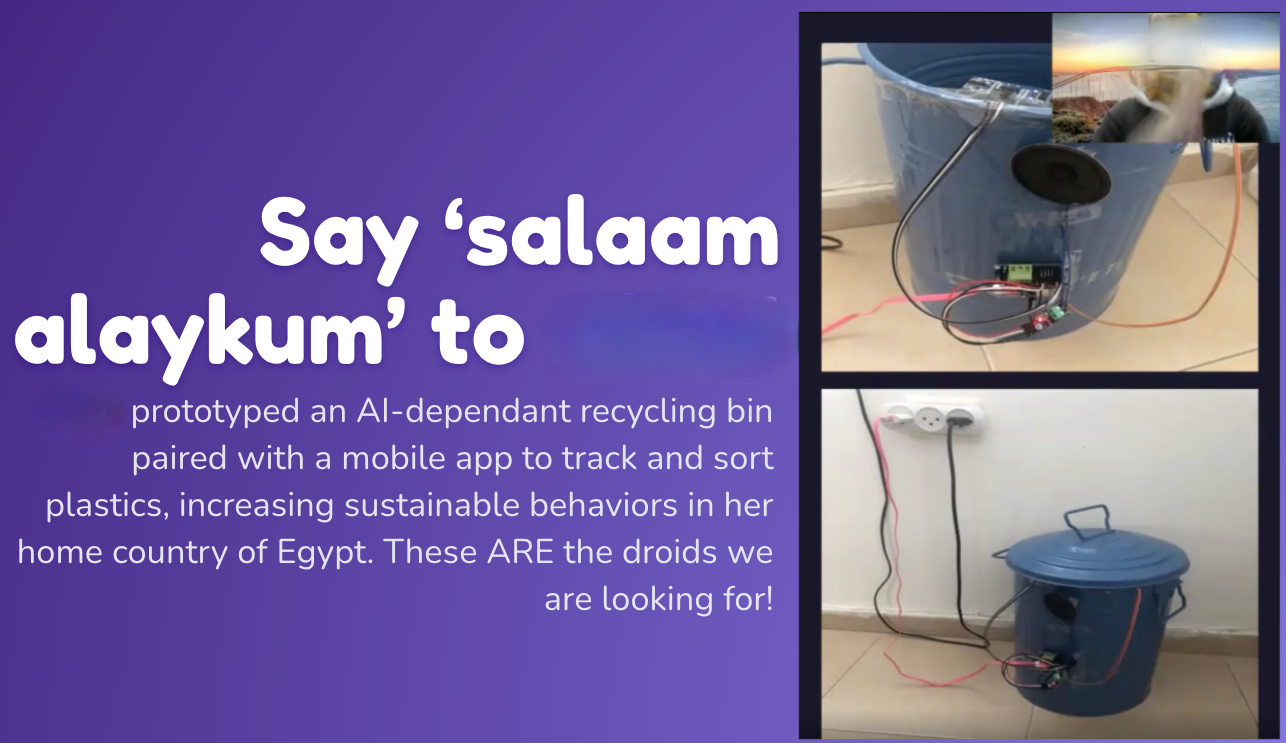
\includegraphics[width=\linewidth]{background/proj1.png}
        \caption{Sample Project 1}
        \label{sfig:can}
    \end{subfigure}
    \hfill
    \vspace{1em}
    \begin{subfigure}{.45\textwidth}
        \centering
        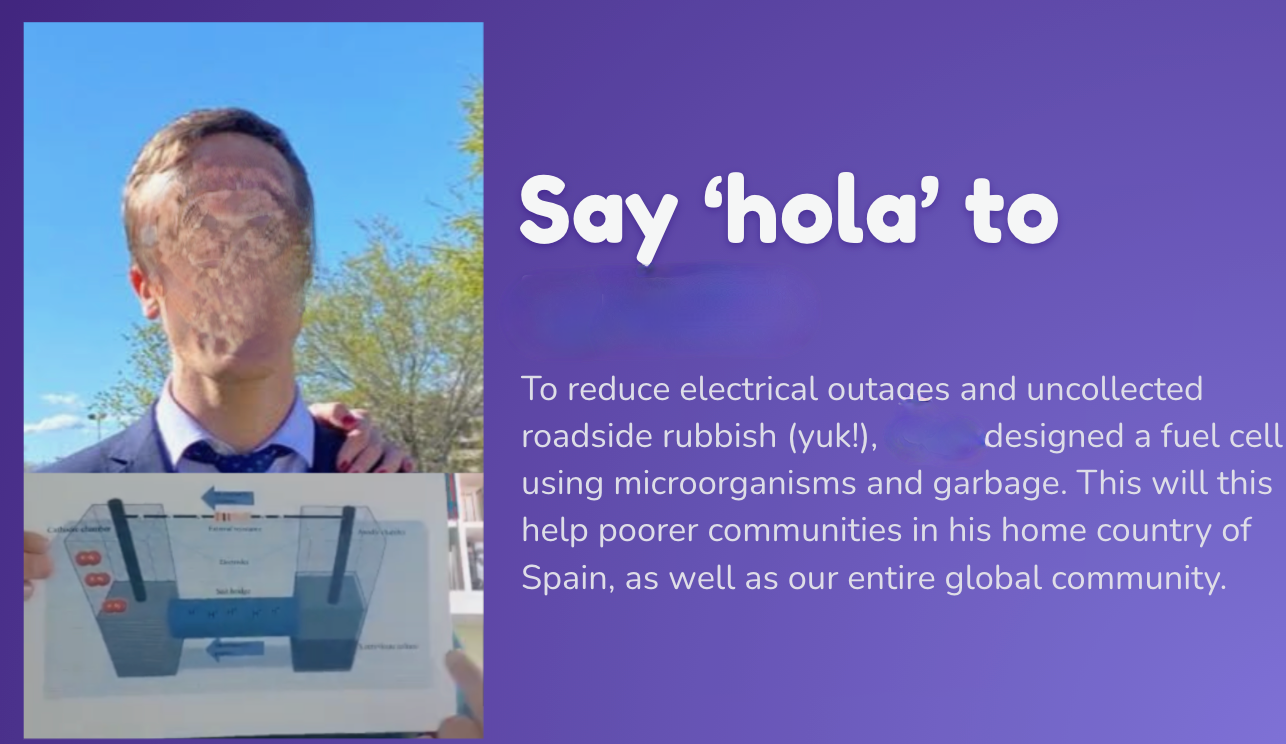
\includegraphics[width=\linewidth]{background/proj2.png}
        \caption{Sample Project 2}
        \label{subfisfigg:cell}
    \end{subfigure}
    \hfill
    \vspace{1em}
    \begin{subfigure}{.45\textwidth}
        \centering
        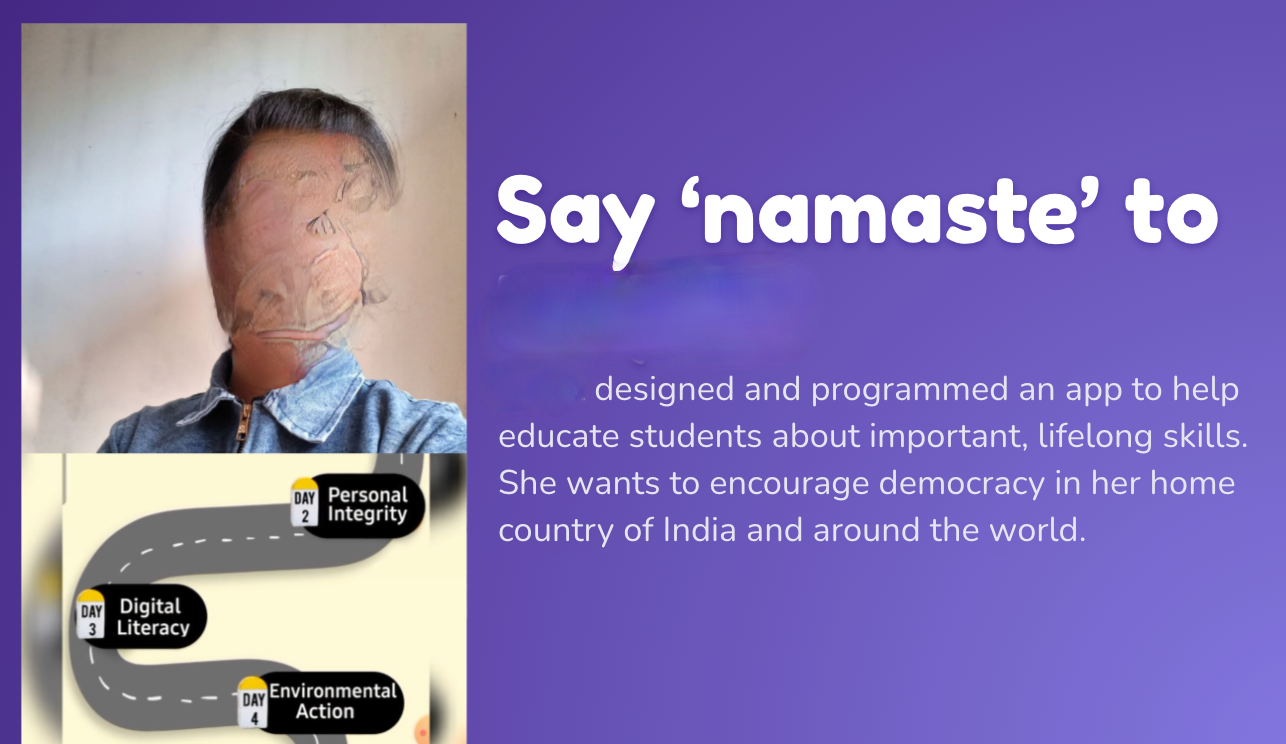
\includegraphics[width=\linewidth]{background/proj3.png} 
        \caption{Sample Project 3}
        \label{sfig:app}
    \end{subfigure}
    \caption{The three panels in this figure depict slides from a program presentation that highlighted three projects that were submitted as part of Rise's 2021 application cycle. Figure \ref{sfig:can} depicts an AI-dependent recycling bin paired with a mobile app to track and sort plastics. Figure \ref{sfig:cell} depicts schematics for a clean fuel cell using microorganisms and garbage. Figure \ref{sfig:app} depicts an app to help education students about the importance of various technical and character skills. Names have been removed and pictures blurred to de-identify program applicants.}
    \label{fig:example_projects}
\end{figure}

Stage one of selection occurs asynchronously (via smartphone, laptop, or, in rare cases, pen and paper) and in two parts. The first part requires applicants to submit an application form with their demographic information and either video or written essays. The first of these two essays explains a real-world problem the applicant wishes to solve, while the second discusses either the ways in which they consider themselves privileged or the challenges they have overcome.\footnote{Refinements to the application process between years all application materials change slightly over time. This change is most dramatic in the case of this second essay, where the focus of the essay changed from an applicant declaration of their own privelege to a description of a challenge the applicant has faced and how they overcame it. Changes appear throughout the application across years; we only detail them where it is relevant to our research.} In the second part, applicants complete a set of digital cognitive assessments and a project showcasing their talent.\footnote{In rare cases, technology or accessibility limitations prevented applicants from completing the cognitive assessment; these applicants were considered on the merits of their submitted materials.} The project showcase is a distinctive part of Rise's selection process whereby particpants: (1) identify a problem they wish to solve, (2) research solutions to that problem, (3) implement those solutions, and (4) reflect on what they learned from the project. Participants submit one essay (video or text) on each of these four stages. Three example projects can be found in Figure \ref{fig:example_projects}. All applicants also submit a short written essay explaining their project and its significance. For an overview of the stage one selection design, see Figure \ref{fig:design}.

\begin{figure}[htbp]
    \centering
    \caption{This figure schematizes the key elements of the talent investment program's data collection and selection process. }
    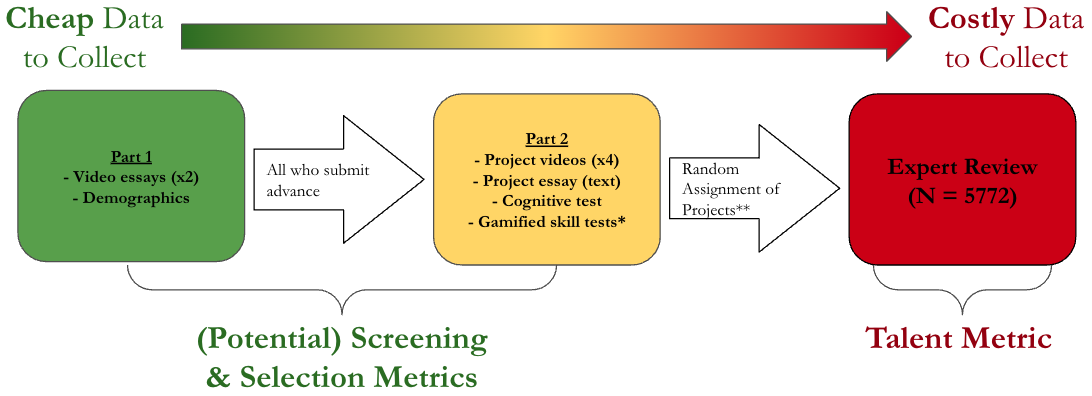
\includegraphics[width=\textwidth,height=\textheight,keepaspectratio]{background/selection_design_schematic.png} 
    \label{fig:design}
\end{figure}

Stage two of selection occurs syncrhonously (though still remotely) in one of several ``finalist days''. The finalist days consist of up to five activities of three types: presentations (where finalists present information about their project), group activities (where finalists collaborate to discuss and solve problems), or interviews (where finalists are interviewed). All activities were judged by a pool of adult `selectors' who assessed finalists according to a rubric. Winner selection decisions were made based both on data collected in stage two and information retained from stage one.

\subsubsection{Program Selection Goals}
- Rise values the 5 traits
- Especially brilliance
- Rise also values diversity

\subsubsection{Data Collection}
Across the application cycle, Rise collects a variety of data from applicants. This data includes traditional merit-based measures – including cognitive tests, written essays, and referrals – as well as non-traditional measures – including peer reviewed video essays, gamified skill tests, and application platform behaviors. Many of these measures are used only for research purposes, and some are tangential to our research on supporting the selection process. We discuss relevant measures here.

% Shorten and rewrite this paragraph (from SPF paper) to suit the thesis.
% Also: the program uses four metrics! Include verbal reasoning!

\paragraph{Cognitive Assessments}
% In all three cycles, applicants took an intelligence test based on the International Cognitive Assessment Resource (ICAR) \cite{condon2014international, subotic2020psychometric}. The full ICAR test is intended to be an accessible and easy-to-understand test that yields a psychometrically validated measure of IQ. Because the program is international, they use only the three item types that are not heavily reliant on English language knowledge: Cube Rotation, Number Sequence, and Matrix Reasoning. All three item types are best described using language from the \hyperlink{https://icar-project.org/types/index.html}{ICAR website}: the Cube Rotation items "present participants with cube renderings and ask participants to identify which of the response choices is a possible rotation of the target stimuli", the Number Sequence items ask participants to "fill in one or two numbers that follow in the sequence", and the Matrix Reasoning items "contain stimuli that are... 3x3 arrays of geometric shapes with one of the nine shapes missing" (similar to those used in Raven's Progressive Matrices) and participants "are instructed to identify which of six geometric shapes presented as response choices will best complete the stimuli". Depictions of each item type are shown in Figure \ref{fig:icar_items}. 

% ICAR scores are generated from estimation of a Bayesian generalized linear item response model following \textcite{burkner2021bayesian}. In particular, define an indicator of whether person $p$'s answer to item $i$ is correct as $\psi_{pi}$. $\psi_{pi}$ is modeled as being determined by a respondent effect -- interpreted as a person $p$'s cognitive ability $\theta_p$ -- and an item effect -- interpreted as the item $i$'s difficulty $\xi_i$. The model also includes and additional \emph{discrimination} parameter $\alpha_i$ which allows items to vary in how well they differentiate high ability vs. low ability respondents. Altogether, this means 

% \begin{equation}
% \psi_{pi} = f\big(\alpha_i(\theta_p + \xi_i)\big). \nonumber
% \end{equation}

% Following the literature, the link function $f(\cdot)$ is logistic, which makes it a general linear model. In particular, we have

% \begin{equation}
% \psi_{pi} = \frac{\mathbb{e}^{\big(\alpha_i(\theta_p + \xi_i)\big)}}{1 + e^{\big(\alpha_i(\theta_p + \xi_i)\big)}}, \nonumber
% \end{equation}

% Which is estimated using Bayesian GLM via \textbf{brms} \textbf{R} package. Bayesian methods were employed to allow the program to utilize prior knowledge from ICAR scoring on meaningfully different, but larger samples. The cognitive ability score assigned to each applicant $p$ for analysis in this paper is the percentile of the median of the posterior distribution of $\theta_p$.

% In addition to ICAR, the program also collected an ability measure from a gamified skills test called Roomworld. Roomworld is intended to measure intelligence and creativity in a way that is fun, novel, and not dependent on culture-specific knowledge. In each level, applicants are challenged to move through the grid using the arrow keys to get the yellow icon to a gift icon. Shapes within the grid serve as different obstacles and mechanisms for navigating the level. How each obstacle and mechanism work are not explained to the player, as part of the test is about discovering how they work. For an example level of the game, see Figure \ref{fig:roomworld_instance}. Multidimensional data from the game are collected and aggregated to give players a percentile score.\footnote{Roomworld was created and scored by an external partner to the program and the specific scoring algorithm was not shared with the authors of this paper.}

\paragraph{Peer Review}
Stage one applicant essays were judged by two types of human evaluators: other applicants (peers) and adults with some expertise on the project topics (experts). Though \textcite{citation needed} provide some evidence for peer review as a measurement of aptitude, peer review was (and remains) experimental, and Rise treated it as such. To collect peer reviews, each applicant was assigned to review 20 of each essay submitted. Each review consisted of Likert scale judgements designed to measure: intelligence, perseverance, empathy, integrity, sense of calling, and impact on the applicant (see Table \ref{tab:rise_measure_details} for details of measurement).

\paragraph{Expert Review} 
Experts, on the other hand, were only asked to assess applicant project essays. Each reviewer was assigned a number of projects proportional to their capacity to review. Like peers, experts were asked to review different elements of the project, using Likert scales to gauge how effective the project was at accomplishing what the applicant intended and how impressive the project was relative to other projects in this field (see Table \ref{tab:rise_measure_details} for details of measurement). 

\paragraph{Finalist Day Activities}
The finalist day activities were assessed by selectors through a mix of qualitative and quantitative measures. Each activity was scored on a rubric, and the scores were aggregated to create a final score for each finalist on each activity type. Additionally, selectors were given an option to provide specific qualitative feedback on applicants.

\subsection{The Ellison Scholars Program}\label{ssec:ellison}
\subsubsection{Program Overview}
Funded and adminsitered by the Ellison Institute of Technology, The Ellison Scholars Program\footnote{https://eit.org/ellisonscholars/} is a global scholarship program that seeks to develop global technology innovators and leaders by finding and supporting talented people passionate about solving humanity’s most serious problems as they study at the University of Oxford and solve global problems through innovation. The program seeks to select at least twenty scholars each year beginning in 2025.

As the Ellison Scholarship's innagural cohort has yet to be selected, program benefits have yet to be dispersed. However, the program has committed to providing scholars with an academic scholarship to the University of Oxford and paid internships. These internships, as well as the program as a whole, are organised around four humane endeavours: (1) Health and Medical Science, (2) Food Security and Sustainable Agriculture, (3) Climate Change and Clean Energy, and (4) Government Innovation and Era of Artificial Intelligence.

\subsection{The Selection Process}
The Ellison Scholarship employs a three-stage selection process. In stage one, applicants submit various application materials asynchronously; the program selects semi-finalists based on the quality of those materials and the program's cohort composition goals. In stage two, semi-finalists apply to the University of Oxford, and the University handles their own internal selection process; program applicants who recieve Oxford scholarships are dubbed Finalists. In stage three, finalists engage in a series of synchronous activities before final decisions are made by the program's board. 

In stage one of selection, applicants submit: their demographic information; selections for humane endeavour, Oxford course, and preferred project; their education record; a list of achievements; and four written essays speaking to their suitability for the program. These essays speak to the applicant's alignment to their chosen humane endeavour, alignemnt to their chosen course at Oxford, and their particular skills and archetype. After submitting this application, all applicants are invited to take a cognitive assessment assessing convergent and divergent reasoning.

In stage two, semi-finalists apply to the University of Oxford; in stage three, finalists engage in a series of synchronous activities before final decisions are made by the program's board. As the Ellison Scholars program is still selecting their innagural cohort, neither stage two nor stage three have been enacted. Thus, we omit details on them here. 

\subsubsection{Program Selection Goals}
- the Ellison Scholars selects around institute projects and humane endeavours
- While many members of the team are sympathetic to demographic diversity, more cognitive definitions are more gemane

\subsubsection{Data Collection}
The Ellison institute collects and constructs a number of different aptitude measurements of applicants. This is primarily traditional merit-based measures, e.g., cognitive tests, written essays, or academic transcripts. Additionally, the program constructs a number of more experimental measures from gathered data. We discuss relevant measures here.

\paragraph{Cognitive Assessments} 
Much like the Rise program, the Ellison Scholarship uses a cognitive assessment based on the International Cognitive Assessment Resource (ICAR) \cite{condon2014international, subotic2020psychometric}. Though the details of implementation differ, both programs use the same four item types and same scoring algorithm.

Additionally, the Ellison Scholarship relies on a divergent thinking assesment based on Guildford's Alternative Uses Task (AUT) \cite{citation needed}. % To-do: more on the aut, including scoring methodology and a sample item.

\paragraph{AI-driven Assessment of Essays}
% To-do: fill this out

\paragraph{Expert Assessment of Applications}


\section{The Social Value of Selection}

\section{The Decision Matrix: A Framework for Understanding Selection Decisions and Evaluating DSTs}
